\documentclass{beamer}
\usetheme{metropolis}
\usepackage{graphicx}
\usepackage{amsmath}
\title{A History of Science in Latin America (INTD290): Unit 0.1}
\author{Jordan Hanson}
\institute{Whittier College Department of Physics and Astronomy}

\begin{document}
\maketitle

\begin{frame}{Course Introduction}
\begin{enumerate}
\item Examination of the syllabus
\item \textit{\textbf{\alert{What is science?}}} Group activity in a moment.
\item Inaugural version of the course
\item Connections 2, Culture 3
\item Logistics made necessary by the pandemic
\item Creating quality writing with outlines, and Coggle.it
\item Introduce terminology
\end{enumerate}
\end{frame}

\section{What is Science?}

\begin{frame}{What is Science?}
\textbf{Have you ever been doing science or math homework, and someone asked you what you were doing?  Have you ever attempted to explain to a family member your courses or major?} \textit{... breakout rooms}
\begin{enumerate}
\item How did you answer?
\item What about your behavior indicated to someone that you were \textit{performing} scientific activity?
\item If a person on a park bench left behind their backpack, and you had to examine its contents, how would you know this was a scientist or mathematician?
\end{enumerate}
\end{frame}

\begin{frame}{What is Science?}
\small
Components for \textbf{humans} to perform science \\ Move items from the lefthand list to the right. \textit{... breakout rooms.}
\rule{10cm}{0.05cm}
\begin{columns}
\begin{column}{0.65\textwidth}
\begin{itemize}
\item Collections of data
\item Specimens from nature
\item Formulation of a hypothesis
\item A general paradigm
\item Instruments for making measurements
\item The five senses
\item A system of writing
\item A system of numbers
\item A group of scientists
\end{itemize}
\end{column}
\begin{column}{0.35\textwidth}
\begin{enumerate}
\item ...
\item ...
\item ...
\item ...
\item ...
\end{enumerate}
\end{column}
\end{columns}
\end{frame}

\begin{frame}{What is Science?}
\small
Determine the items at left at work in the following events: \\ \textit{... breakout rooms.}
\rule{10cm}{0.05cm}
\begin{columns}
\begin{column}{0.65\textwidth}
\begin{itemize}
\item Collections of data
\item Specimens from nature
\item Formulation of a hypothesis
\item A general paradigm
\item Instruments for making measurements
\item The five senses
\item A system of writing
\item A system of numbers
\item A group of scientists
\end{itemize}
\end{column}
\begin{column}{0.35\textwidth}
Determine the items at left at work in the following events:
\begin{enumerate}
\item Galileo determining that objects fall at the same rate regardless of mass
\item Aztec doctors determining that chinaberry bark cures syphilis
\end{enumerate}
\end{column}
\end{columns}
\end{frame}

\begin{frame}{What is Science?}
\small
Determine the items at left at work in the following events: \\ \textit{... breakout rooms.}
\rule{10cm}{0.05cm}
\begin{columns}
\begin{column}{0.65\textwidth}
\begin{itemize}
\item Collections of data
\item Specimens from nature
\item Formulation of a hypothesis
\item A general paradigm
\item Instruments for making measurements
\item The five senses
\item A system of writing
\item A system of numbers
\item A group of scientists
\end{itemize}
\end{column}
\begin{column}{0.35\textwidth}
\begin{enumerate}
\item Incan accountants devising \textit{quipu} knots to record taxation information in their Andean provinces\footnote{Is this science?  If not, what is it?}
\item Aztec doctors determining that chinaberry bark cures syphilis
\end{enumerate}
\end{column}
\end{columns}
\end{frame}

\begin{frame}{What is Science?}
\begin{figure}
\centering
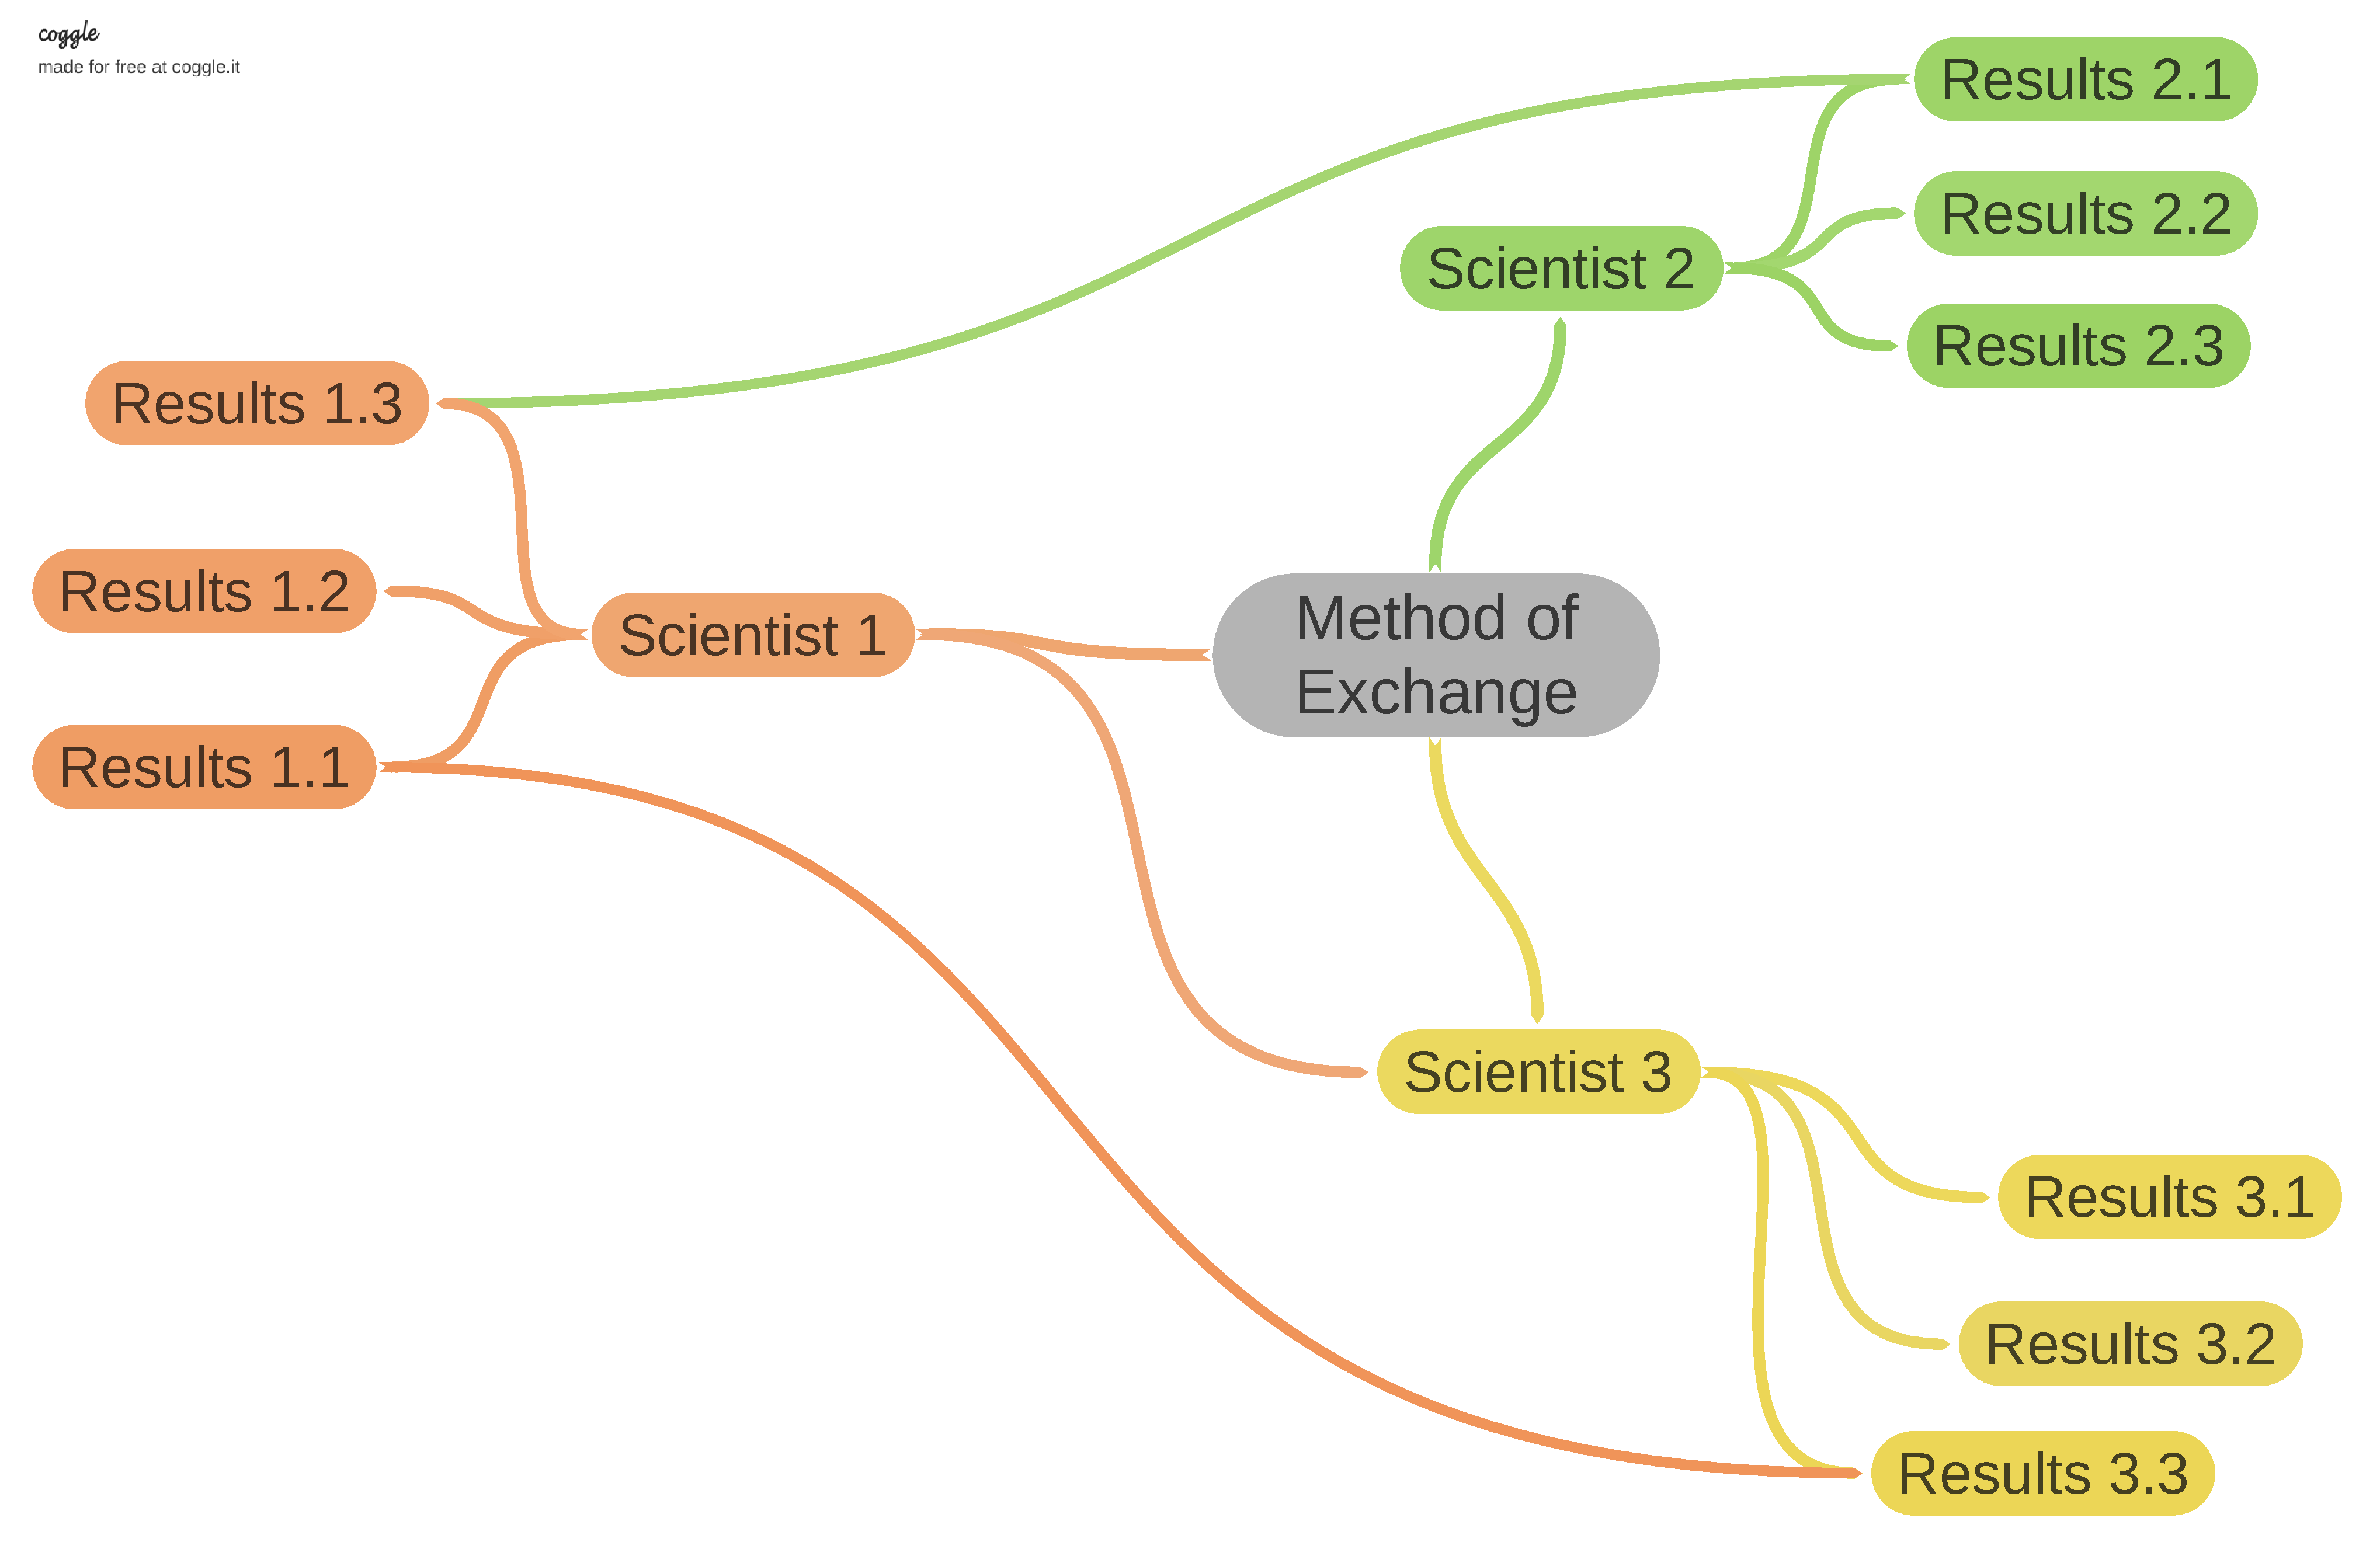
\includegraphics[width=10cm]{figures/ScientificExchange.pdf}
\caption{An imperfect method of exchange in a scientific community.}
\end{figure}
\end{frame}

\begin{frame}{What is Science?}
\begin{figure}
\centering
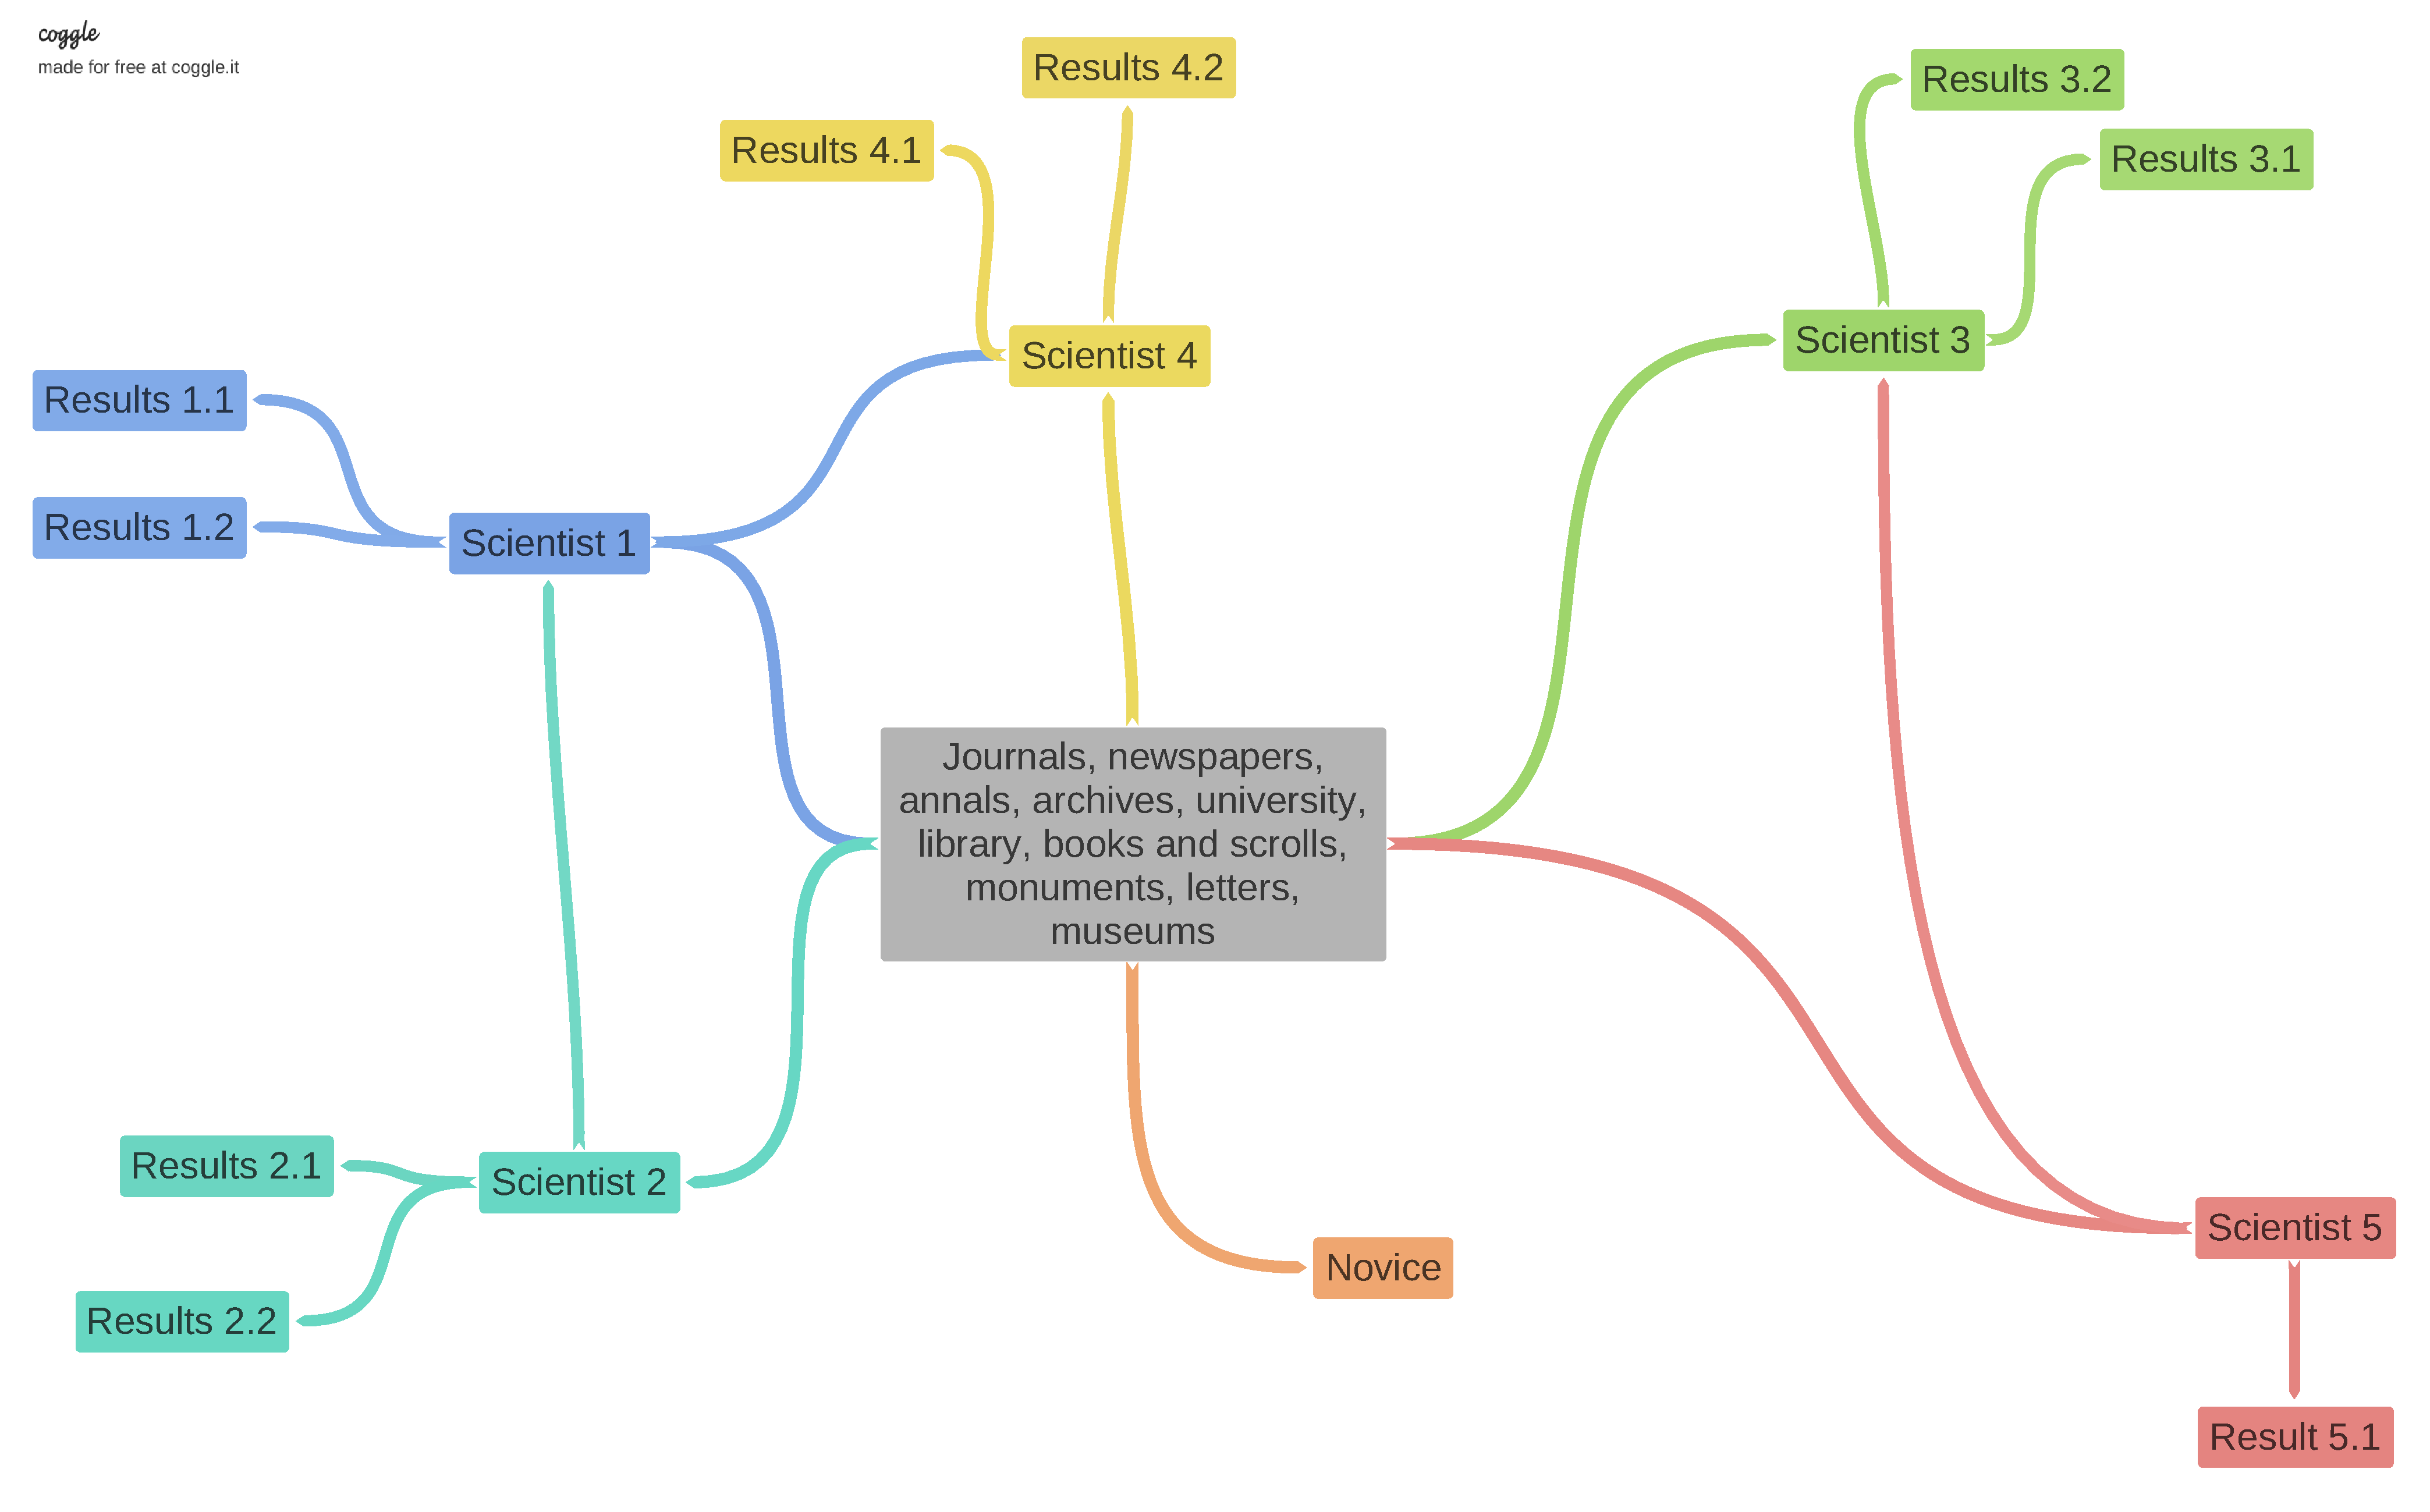
\includegraphics[width=10cm]{figures/ScientificExchange2.pdf}
\caption{A (less) imperfect method of exchange in a scientific community.}
\end{figure}
\end{frame}

\begin{frame}{What is Science?}
\small
\begin{figure}
\centering
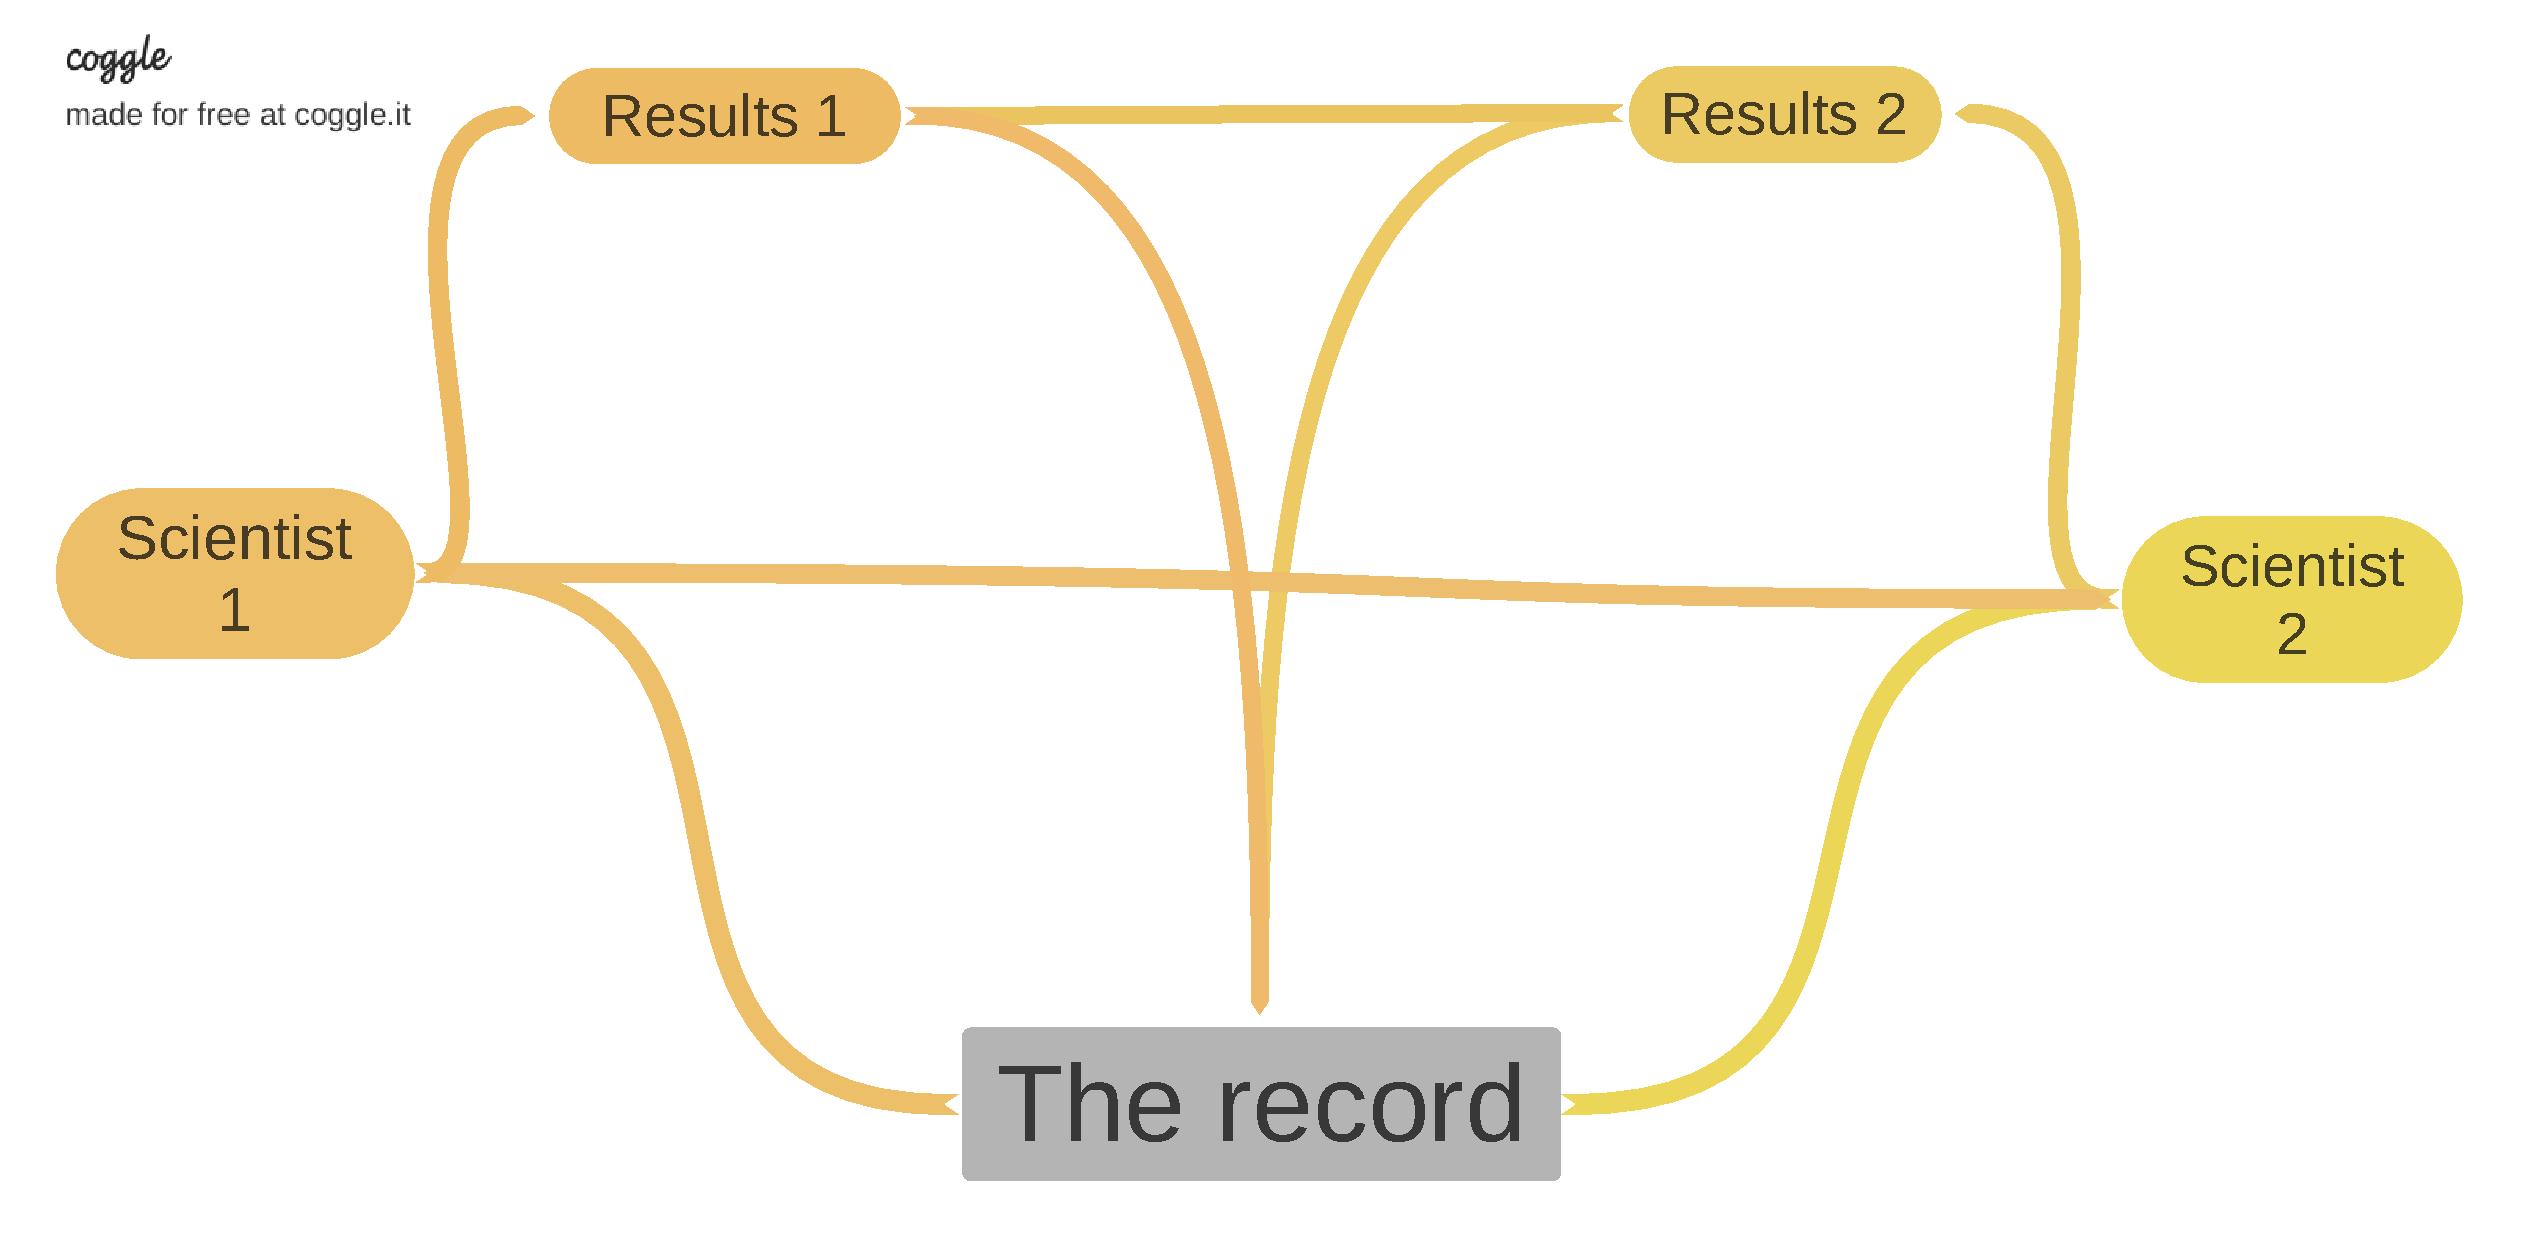
\includegraphics[width=6cm]{figures/ScientificExchange3.pdf}
\caption{An ideal method of exchange in a scientific community.}
\end{figure}
Do we reach this in the modern era?
\begin{enumerate}
\item Traditions of physics in the United States, Russia, and China
\item The internet, computation and large data sets
\item Open-source technologies and strategies
\item Economic trends
\end{enumerate}
\end{frame}

\section{Is Science True?}

\begin{frame}{Is Science True?}
\small
Determine which of the following questions can be answered scientifically, and add them to the list at right \textit{... breakout rooms.}
\rule{10cm}{0.05cm}
\begin{columns}
\begin{column}{0.65\textwidth}
\begin{itemize}
\item What is the nature of time?
\item What colors are present in sunlight?
\item Given market demand, at what price shoud we sell our milk?
\item What is the speed of sound in a particular substance?
\item Are these two individuals related?
\item Are these two individuals in love?
\item What is the arrangement of the Earth, stars, and planets?
\end{itemize}
\end{column}
\begin{column}{0.35\textwidth}
\begin{enumerate}
\item ...
\item ...
\item ...
\item ...
\end{enumerate}
\end{column}
\end{columns}
\end{frame}

\begin{frame}{Is Science True?}
For each question we claim is answerable with the scientific method, think about how we rely on our senses. \\ \vspace{0.5cm}
\textit{What colors are present in sunlight?} Using a prism, we can tease apart the different frequencies of light wave in regular sunlight.
\begin{figure}
\centering
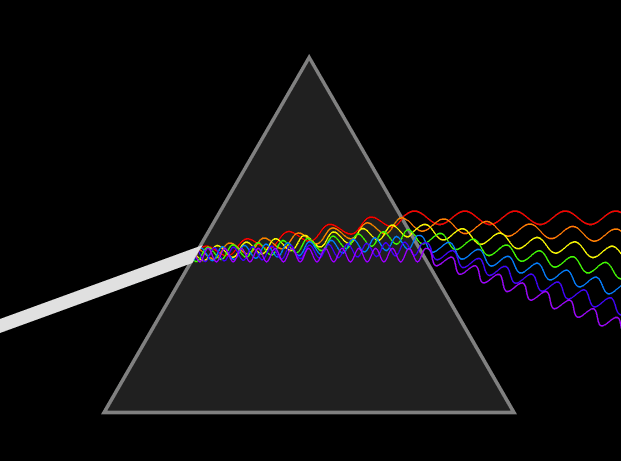
\includegraphics[width=4cm]{figures/prism.png}
\caption{A prism has an index of refraction that depends on the frequency of the light.}
\end{figure}
\end{frame}

\begin{frame}{Is Science True?}
For each question we claim is answerable with the scientific method, think about how we rely on our senses. \\ \vspace{0.5cm}
\textit{What colors are present in sunlight?}
\begin{figure}
\centering
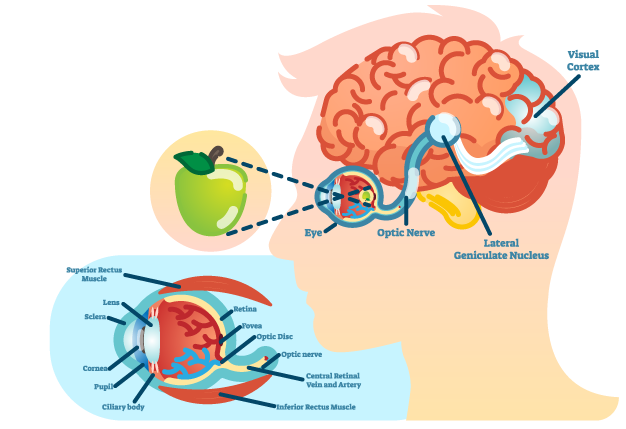
\includegraphics[width=5cm]{figures/eye.png}
\caption{However, the light is still something you perceive with your eyes.  The eyes are merely producing electrical signals after focusing the light.}
\end{figure}
\end{frame}

\begin{frame}{Is Science True?}
For each question we claim is answerable with the scientific method, think about how we rely on our senses. \\ \vspace{0.5cm}
\textit{What colors are present in sunlight?}
\begin{figure}
\centering
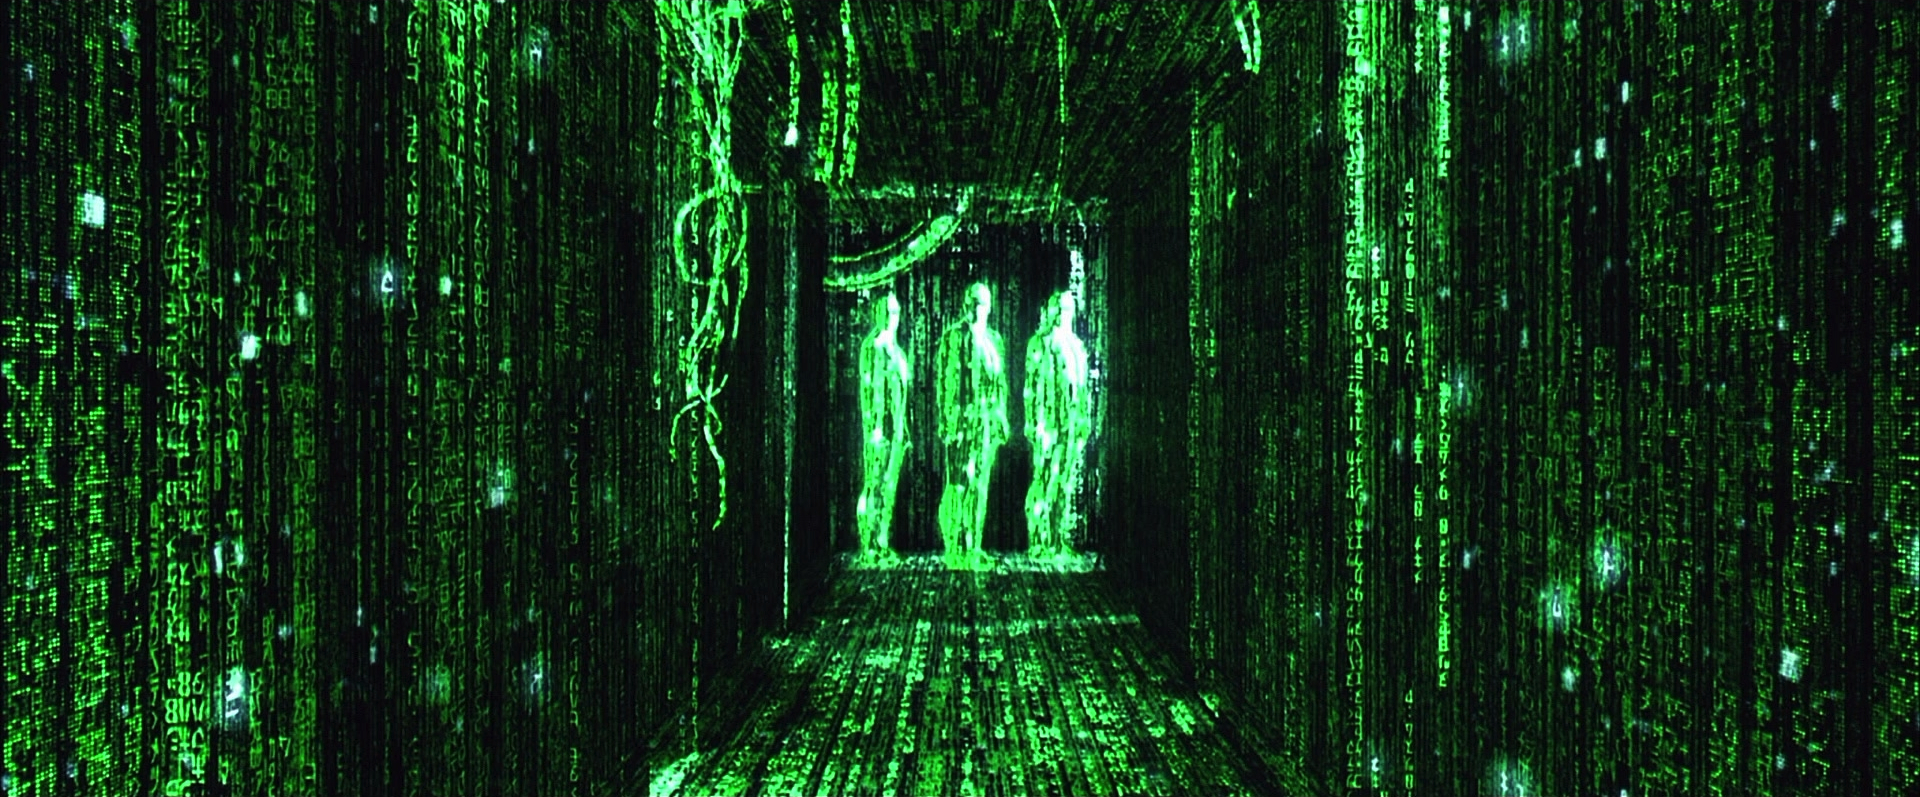
\includegraphics[width=7cm]{figures/matrix.jpg}
\caption{And if your eyes are optical devices that produce electrical signals, how do you know that the actual universe appears the way you think it does?  Is it possible that the signals that serve as input to your perception are from somewhere else? The matrix ...}
\end{figure}
\end{frame}

\begin{frame}{Is Science True?}
For each question we claim is answerable with the scientific method, think about how we rely on our senses. \\ \vspace{0.5cm}
\textit{What colors are present in sunlight?}
\begin{figure}
\centering
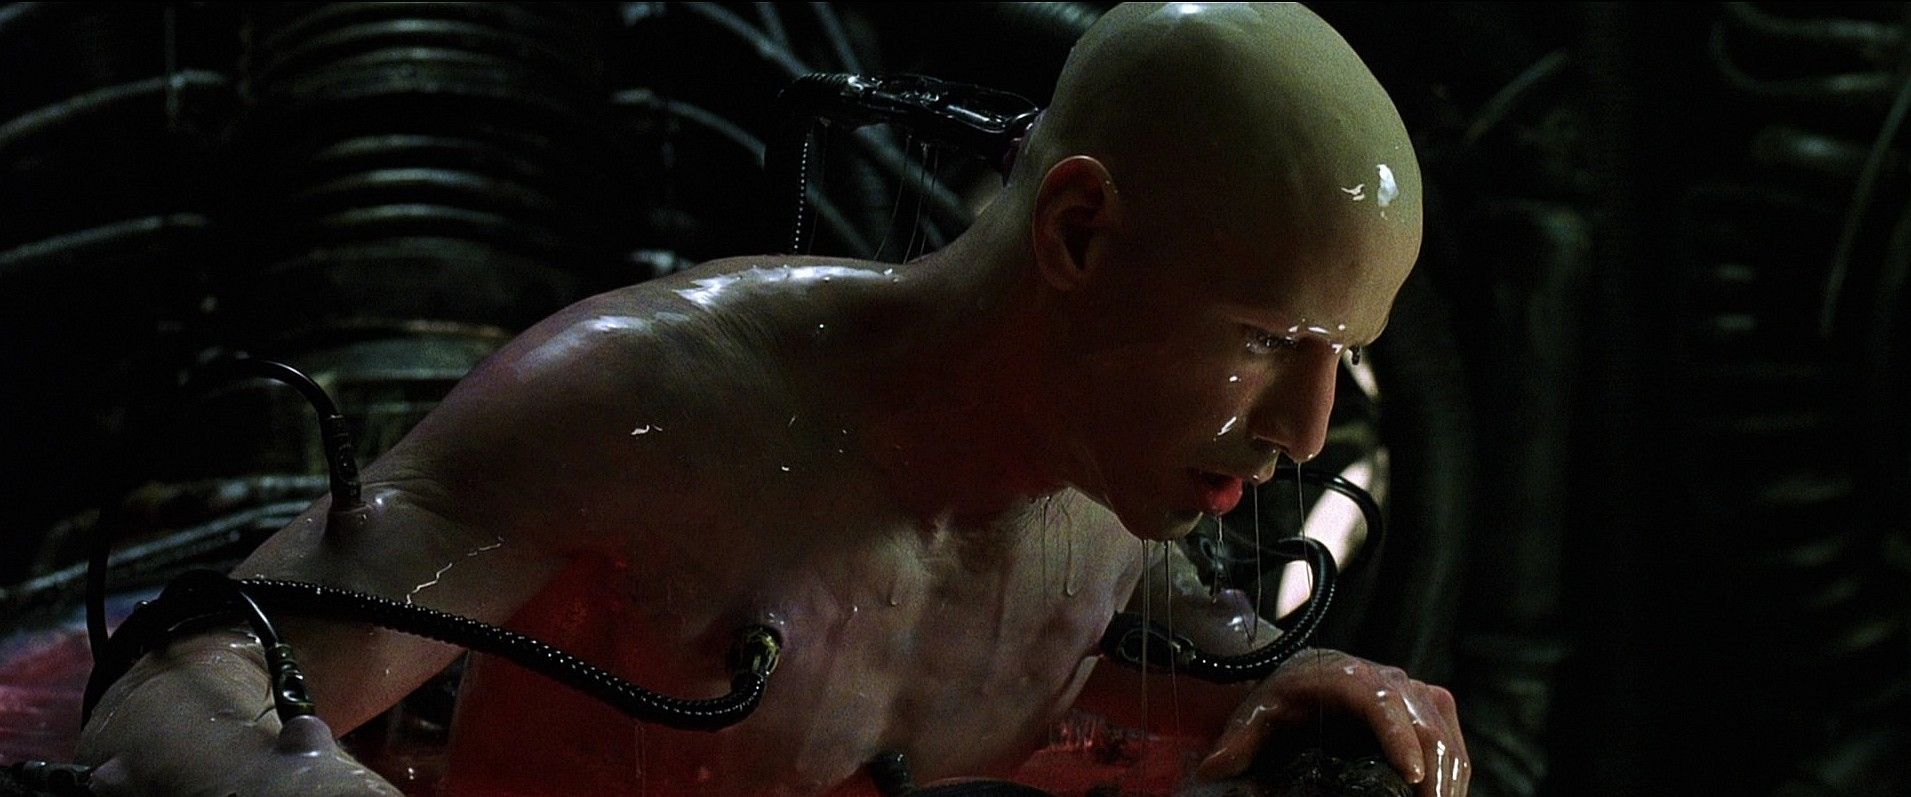
\includegraphics[width=7cm]{figures/matrix2.jpg}
\caption{In this film, the matrix is a complex system delivering electrical signals to the brains and nervous systems of captive human beings.  They have to realize that reality is actually a simulation.}
\end{figure}
\end{frame}

\begin{frame}{Is Science True?}
For each question we claim is answerable with the scientific method, think about how we rely on our senses. \\ \vspace{0.5cm}
\textit{What colors are present in sunlight?}
\begin{figure}
\centering
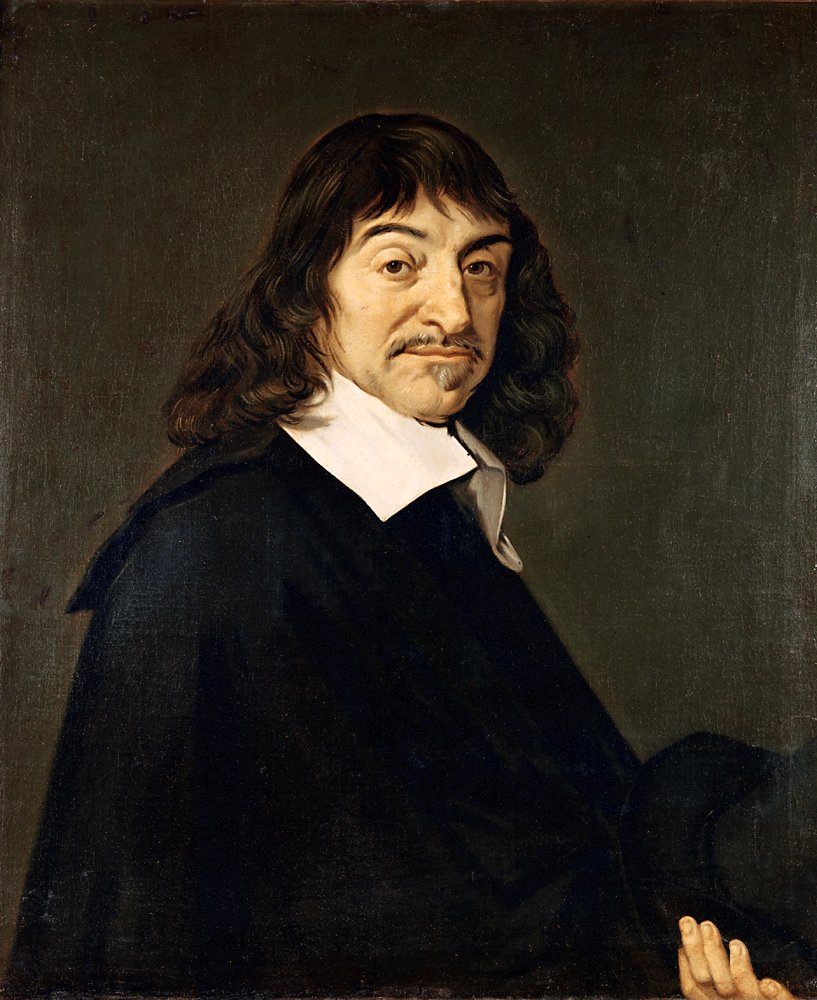
\includegraphics[width=3cm]{figures/rene.jpg}
\caption{A portrait of Ren\'{e} Descartes, French philosopher, mathematician, and scientist, 1596-1650.  You will read about the \textit{Cartesians}, or those that follow his philosophical treatises.}
\end{figure}
\end{frame}

\begin{frame}{Is Science True?}
\small
\begin{enumerate}
\item \textit{Discourse on the Method}\footnote{Discours de la Méthode Pour bien conduire sa raison, et chercher la vérité dans les sciences, 1637}
\begin{itemize}
\item ``I think, therefore I am.''  The method of starting with doubt and finding one concrete thing in which to place belief, before moving forward.
\item Offers three proofs of the existence of God
\end{itemize}
\item An appendix to The Discourse was entitled \textit{Geometry}, which unified algebra and geometry.  This method of translating geometric areas and volumes into algebraic equations was unique and new at the time.  From this moment we get the notion of a coordinate system: Cartesian coordinates
\item Also discussed cosmology, optics, and the psychology of emotions
\end{enumerate}
\end{frame}

\begin{frame}{Is Science True?}
For each question we claim is answerable with the scientific method, think about how we rely on our senses. \\ \vspace{0.5cm}
Some vocabulary:
\begin{enumerate}
\item Epistemology: the theory of the origin of knowledge, distinguishing justified belief from opinion
\item Rationalism: the theory that reason rather than experience is the foundation of certainty in knowledge
\item Empiricism: the theory that all knowledge is derived from sensory experience, stimulated by the rise of experimental science
\item Theology: the study of the nature of God and religious belief, systematically developed
\end{enumerate}
\end{frame}

\begin{frame}{Is Science True?}
For each question we claim is answerable with the scientific method, think about how we rely on our senses. \\ \vspace{0.5cm}
Empiricism: epistemology based on sensory experience.
\begin{enumerate}
\item Clearly has implications for experimental science
\item Modern science (physics) is divided into two poles: \textit{theoretical} and \textit{experimental}
\item Mathematics can be grouped into various categories as well (some didn't exist at the time).
\end{enumerate}
\end{frame}

\begin{frame}{Is Science True?}
\textit{Why does a spring oscillate?  Can we predict the motion?}
\begin{figure}
\centering
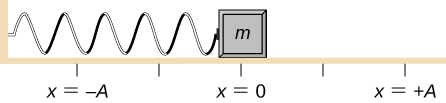
\includegraphics[width=3cm]{figures/spring1.jpeg}
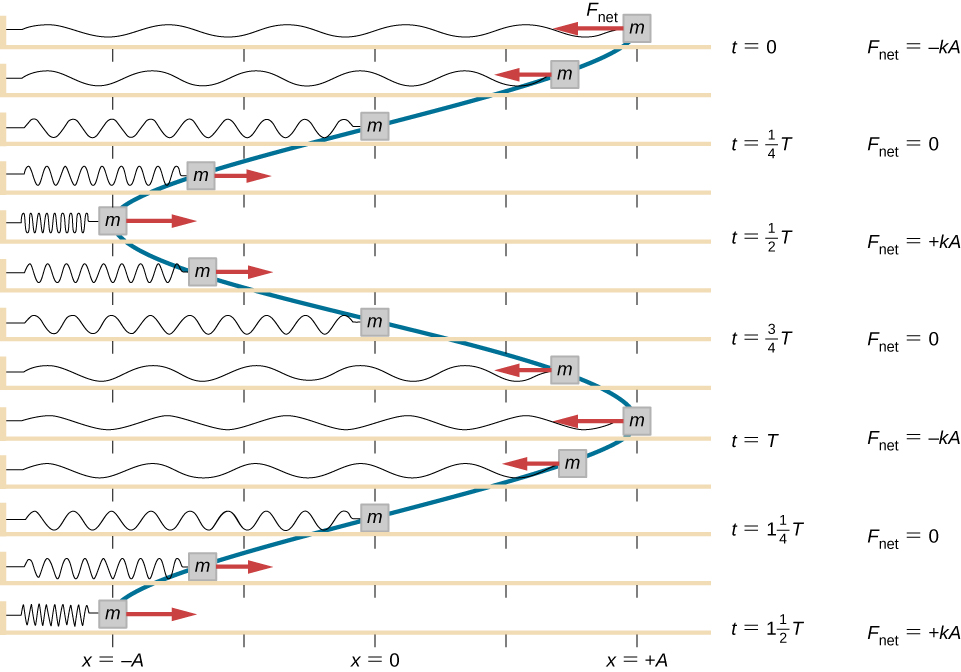
\includegraphics[width=5cm]{figures/spring2.jpeg}
\caption{Springs are subject to Hooke's law, which states that the force is linearly proportional to the change in length of a system.}
\end{figure}
\begin{align}
F &= m \ddot{x} \\
x(t) &= A \cos(\omega t)
\end{align}
\end{frame}

\begin{frame}{Is Science True?}
\textbf{Is this like seeing the future?} - topic of \textit{determinism.}
\begin{figure}
\centering
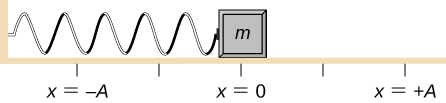
\includegraphics[width=3cm]{figures/spring1.jpeg}
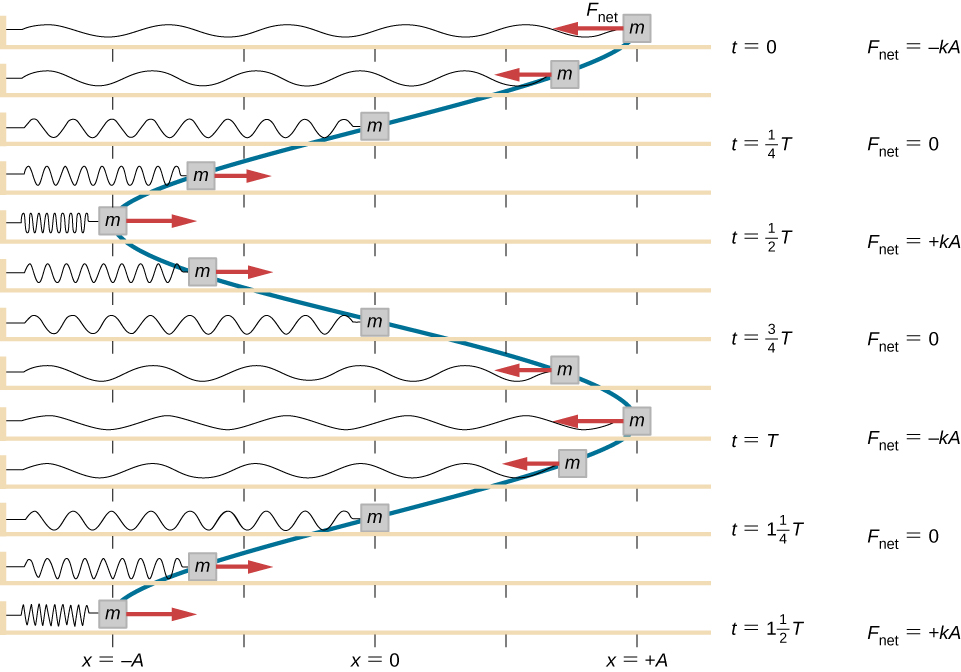
\includegraphics[width=5cm]{figures/spring2.jpeg}
\caption{Springs are subject to Hooke's law, which states that the force is linearly proportional to the change in length of a system.}
\end{figure}
\end{frame}

\section{Catholic Terminology}

\begin{frame}{Catholic Terminology}
\begin{figure}
\centering
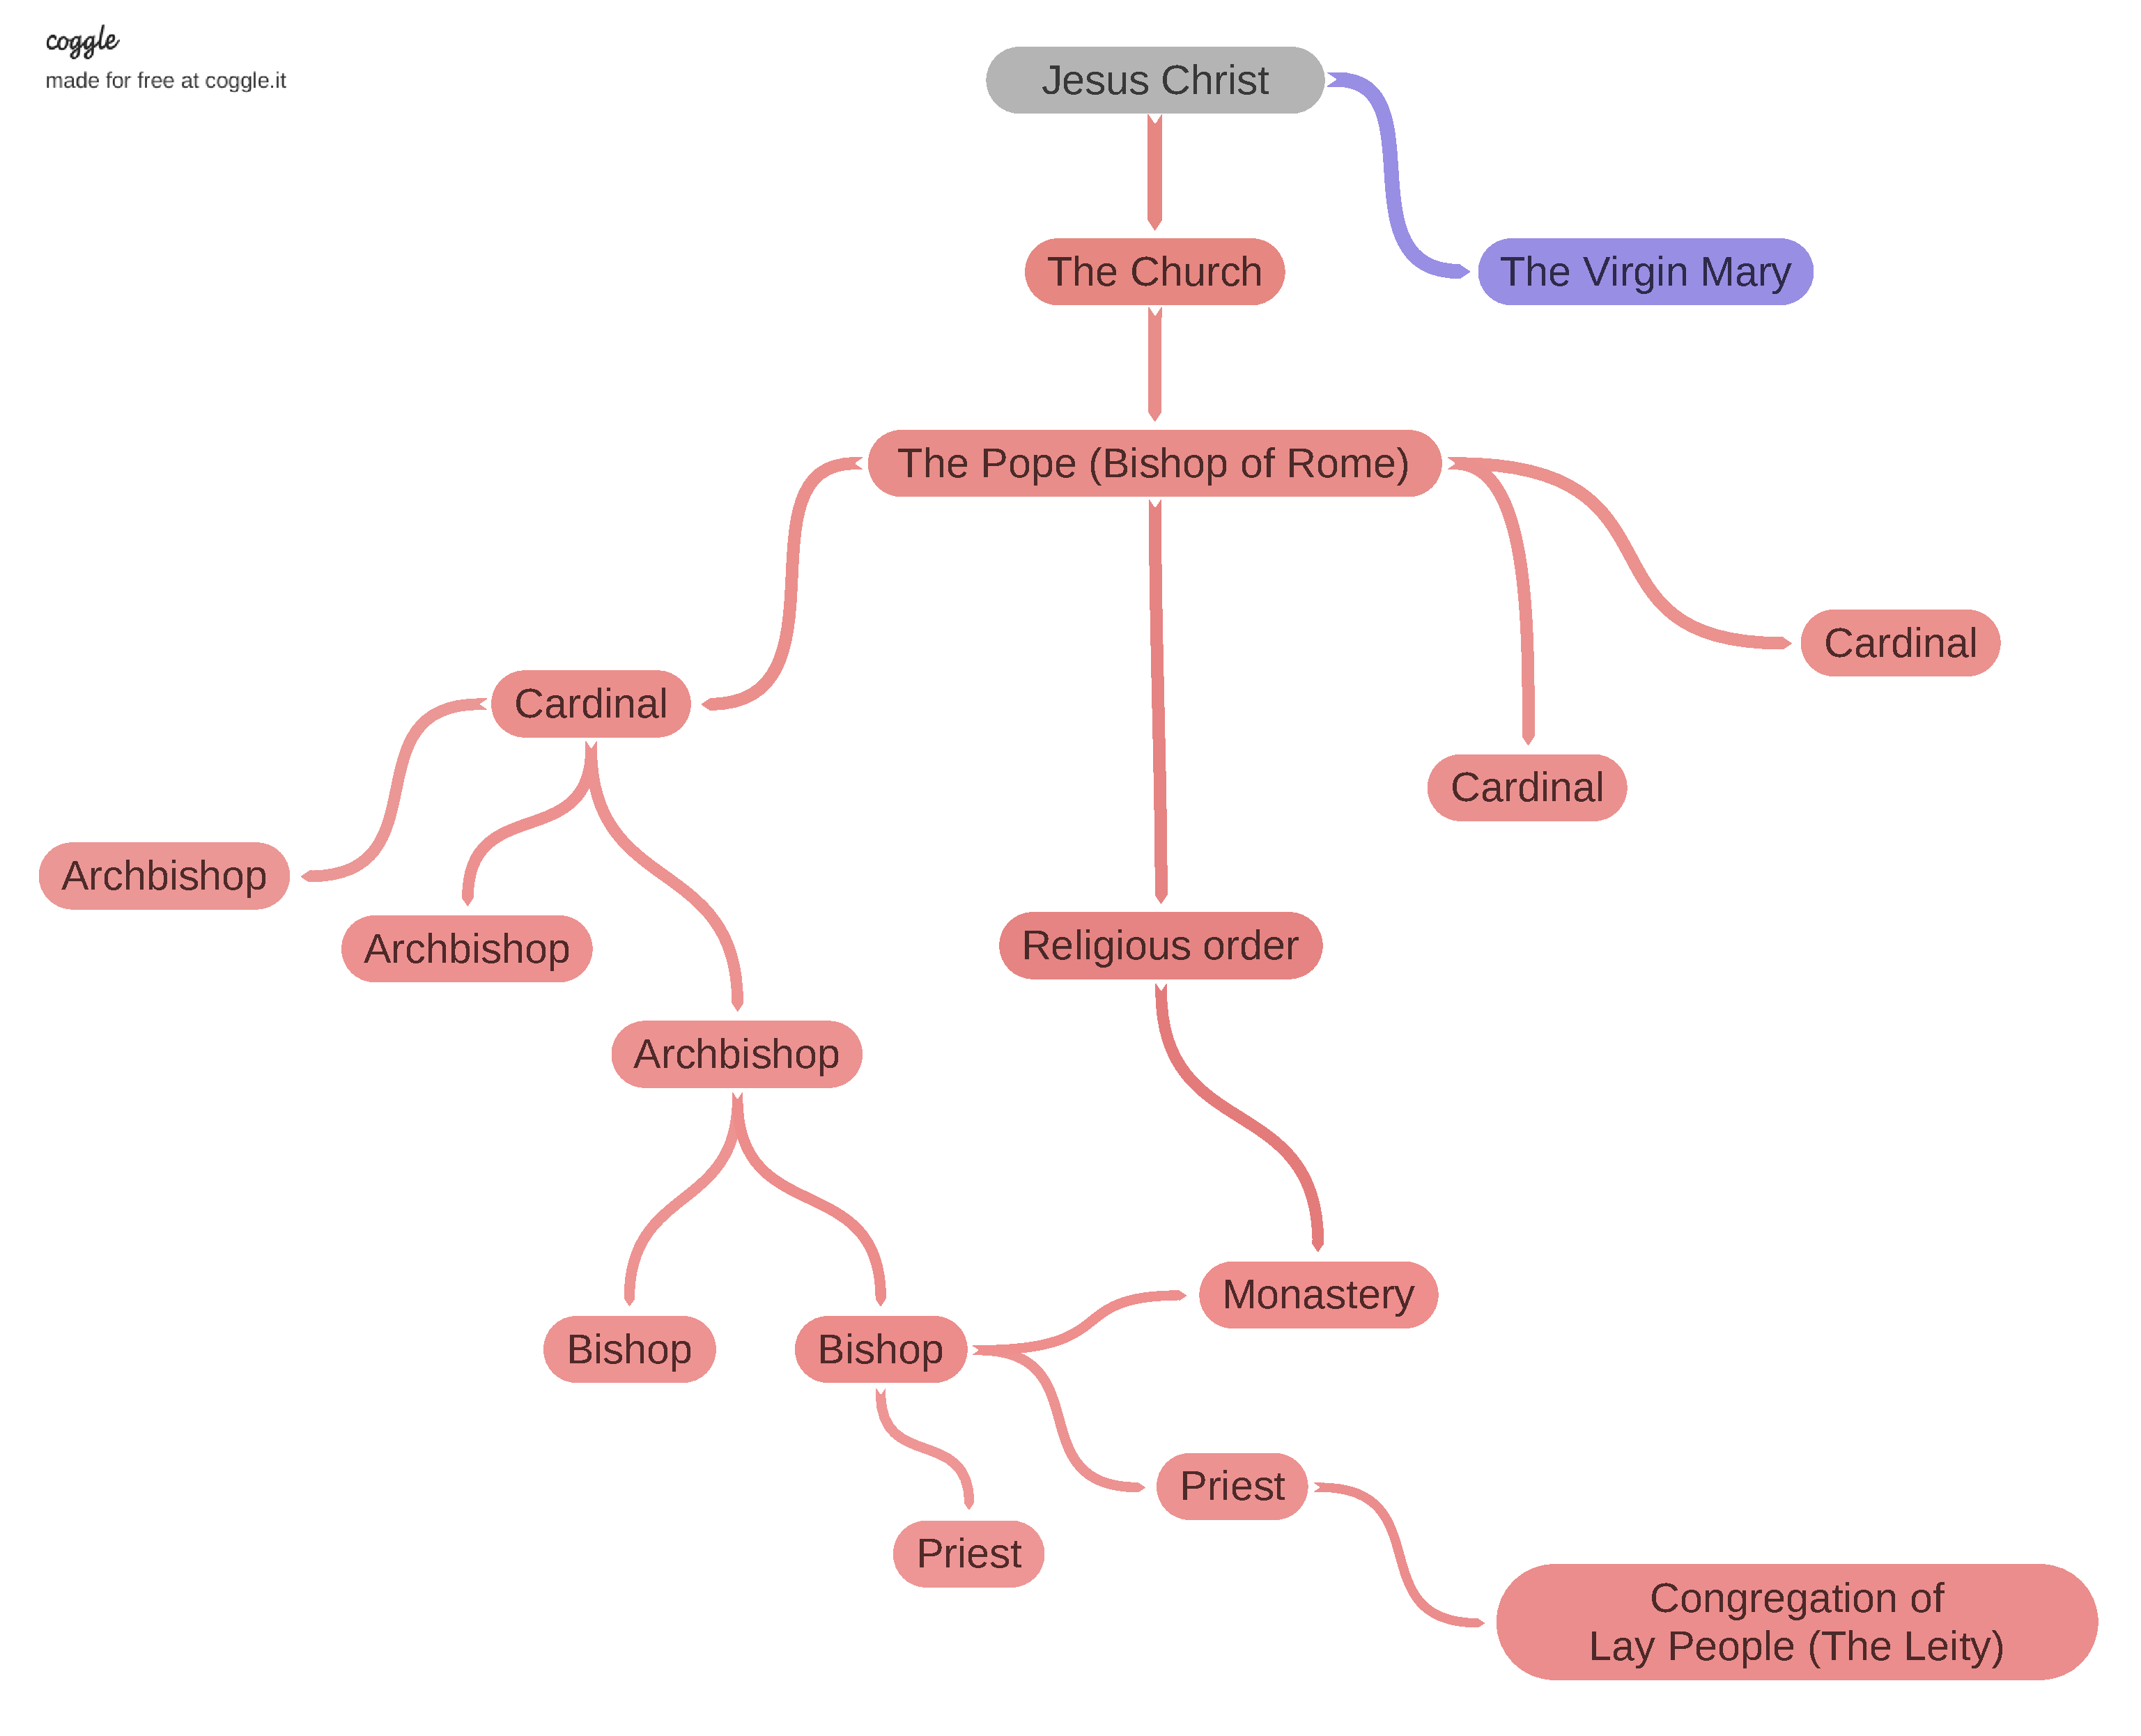
\includegraphics[width=7cm]{figures/catholic.pdf}
\caption{A rough outline of the Catholic Church hierarchy, including \textit{Religious Orders.}}
\end{figure}
\end{frame}

\begin{frame}{Catholic Terminology}
\small
Other Catholic terminology:
\begin{enumerate}
\item Diocese: A district under the pastoral care of a bishop.  A diocese may have several churches or a cathedral, in which people worship.
\item Monastery: A place where those who have taken religious vows (think monks and nuns) live and work.
\item The Society of Jesus (Jesuits): A religious order that played a significant international role in education
\item The Dominican Order: A religious order primarily known for scholastic tradition and preaching the gospel, dealing with heresy
\item Heresy: When a person spreads an idea counter to the teaching of Christ.  For example, the Arian heresy took place in first few centuries in Church history.  The Emperor Constantine attempted to settle the question at the Council of Nicea, from which we get the Nicean Creed.
\end{enumerate}
\end{frame}

\section{Geographic Terminology}

\begin{frame}{Geographic Terminology}
\begin{figure}
\centering
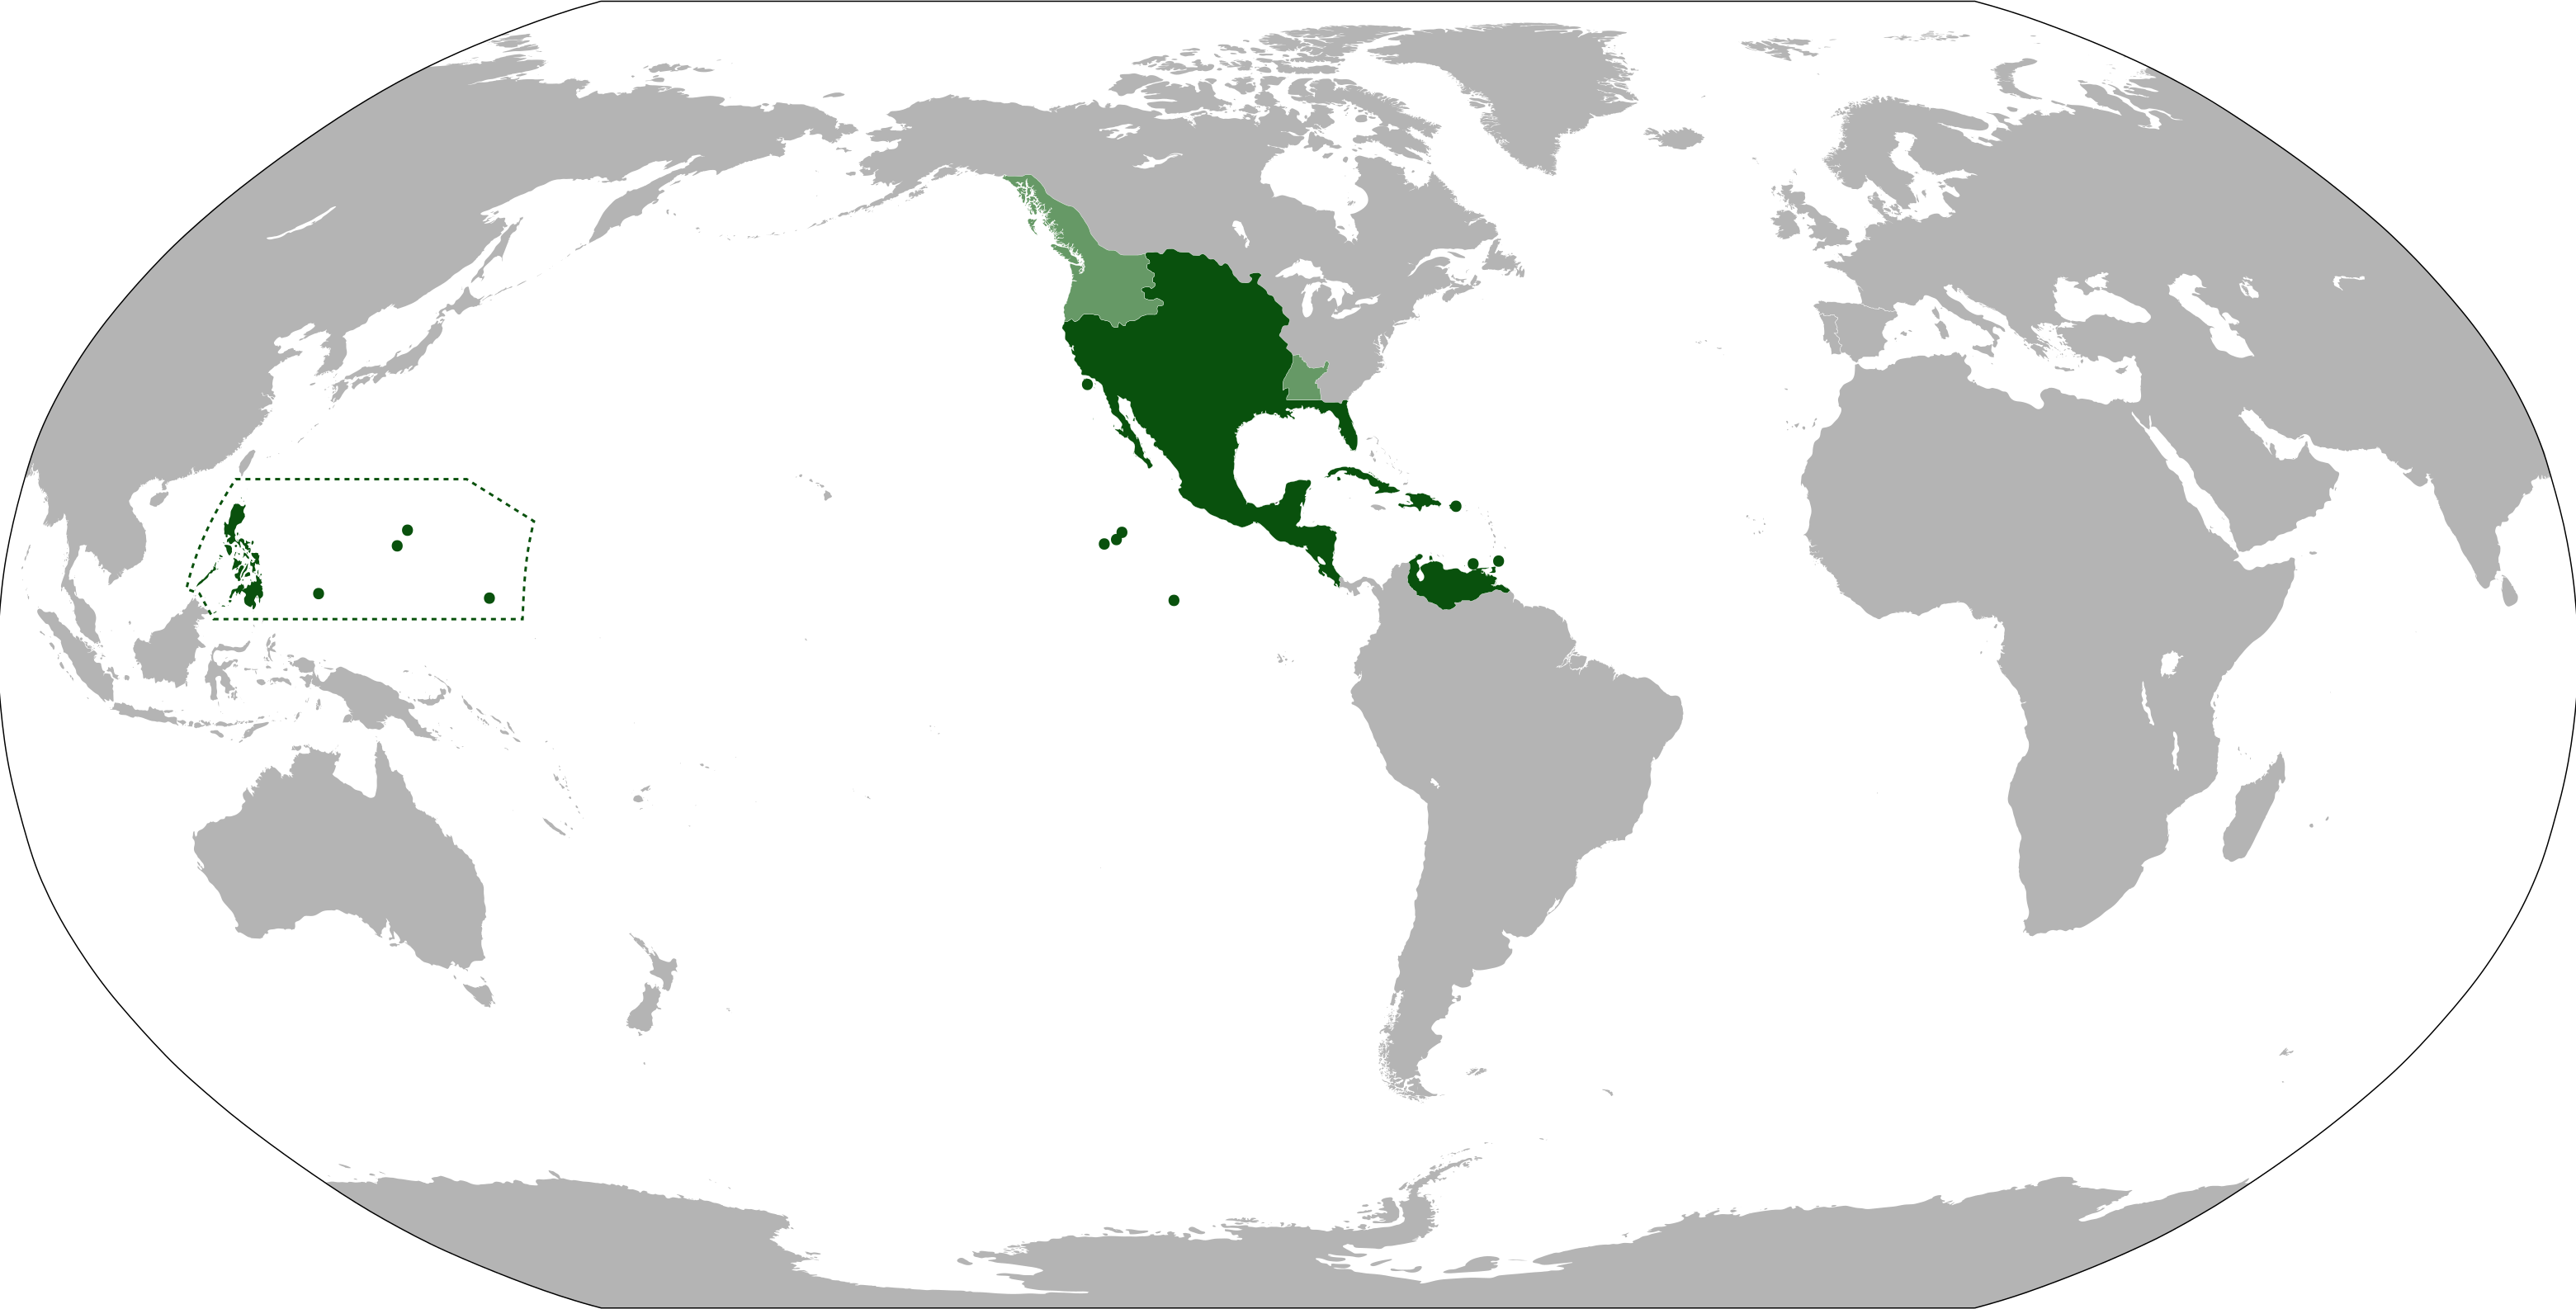
\includegraphics[width=10cm]{figures/vice.png}
\caption{The largest extent of the Spanish colonies in America, up to 1803.}
\end{figure}
\end{frame}

\begin{frame}{Geographic Terminology}
\small
The four major Spanish \textit{viceroyalties}:
\begin{itemize}
\item Virreinato de Nueva Espa\~{n}a, comprised of former Aztec capital and territory
\begin{enumerate}
\item Capital: Ciudad de M\'{e}xico, Tenotchitlan, modern Mexico City
\end{enumerate}
\item Virreinato del Per\'{u}, comprised of former Incan capital and territory
\begin{enumerate}
\item Captial: Lima, Per\'{u}.  The original capital of the Incans was Cusco.  \textit{Note: Incan empire was the largest in the world at the time.}
\end{enumerate}
\item Virreinato de Nueva Granada (from Per\'{u})
\begin{enumerate}
\item Capital: Santa Fe de Bogot\'{a}, modern Bogot\'{a}, Colombia
\item Caracas and Quito are also within this province
\end{enumerate}
\item Virreinato del R\'{i}o De la Plata (from Per\'{u})
\begin{enumerate}
\item Capital: Buenos Aires
\item Modern Argentina, Chile, Bolivia, Paraguay and Uruguay
\end{enumerate}
\end{itemize}
\end{frame}

\begin{frame}{Geographic Terminology}
\begin{figure}
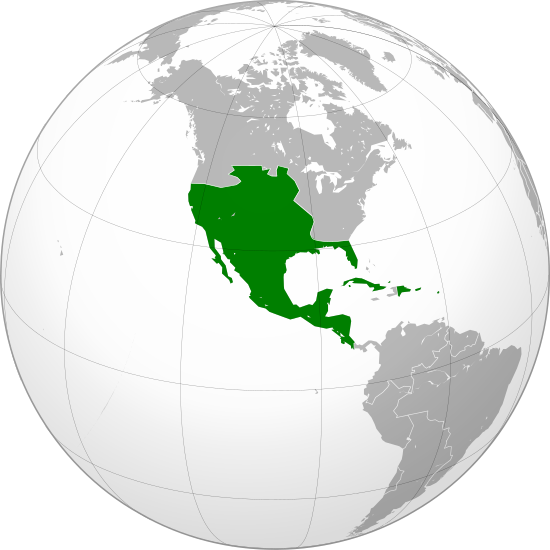
\includegraphics[width=6cm]{figures/vice_nuevaespana.png}
\caption{Virreinato de Nueva Espa\~{n}a}
\end{figure}
\end{frame}

\begin{frame}{Geographic Terminology}
\begin{figure}
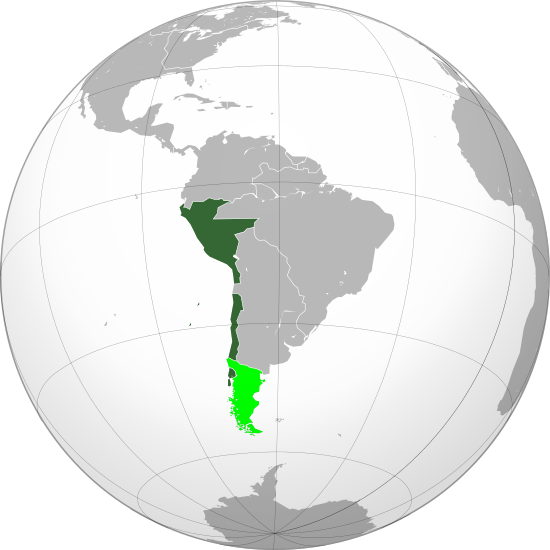
\includegraphics[width=6cm]{figures/vice_peru.png}
\caption{Virreinato del Per\'{u}}
\end{figure}
\end{frame}

\begin{frame}{Geographic Terminology}
\begin{figure}
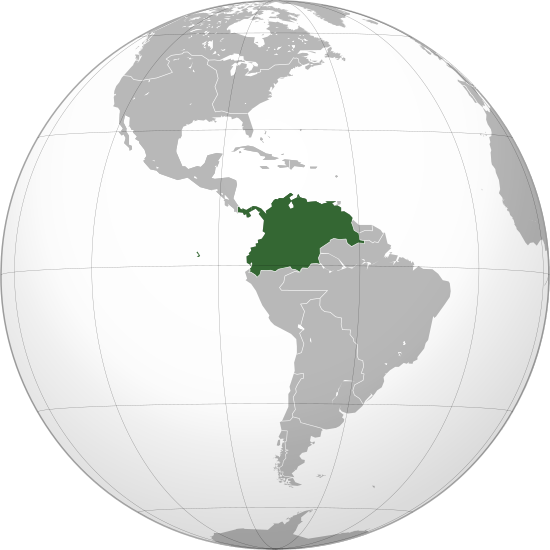
\includegraphics[width=6cm]{figures/vice_nuevagranada.png}
\caption{Virreinato de Nueva Granada}
\end{figure}
\end{frame}

\begin{frame}{Geographic Terminology}
\begin{figure}
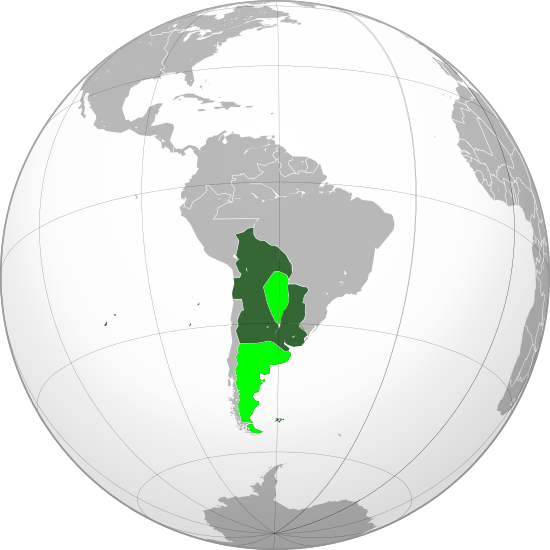
\includegraphics[width=6cm]{figures/vice_riodelaplata.png}
\caption{Virreinato del R\'{i}o De la Plata}
\end{figure}
\end{frame}

\section{Vocabulary: Nahuatl and Espa\~{n}ol}

\begin{frame}{Vocabulary}
\small
Nahuatl vocabulary\footnote{The letter x makes a sound much like the English ``h,'' as in \textit{M\'{e}xico} or \textit{Oaxaca}.}:
\begin{enumerate}
\item \textbf{Nahua}: main ethnic group indigenous to Mexico.  The Aztecs were of Nahua ethnicity.  Around 500 BC, settled in the basin in central Mexico.
\item \textbf{Nahautl}: a language group of the Nahua
\item \textbf{altepetl}: a Nahua city-state within which most individuals were of the same tribe and ethnicity.  Sub-unit: \textbf{calpolli.}
\item \textbf{amoxtli}: a codex or book written in Nahuatl
\item \textbf{tlacuiloll}: a painting or stelae
\item \textbf{tlacuilo}: one who paints or records, a notary or scribe
\end{enumerate}
\end{frame}

\begin{frame}{Vocabulary}
\small
Nahuatl vocabulary\footnote{The letter x makes a sound much like the English ``h,'' as in \textit{M\'{e}xico} or \textit{Oaxaca}.}:
\begin{enumerate}
\item \textbf{Nahuatl list of animals}: \url{http://www.native-languages.org/nahuatl_animals.htm}. \textit{Nota bene: la historia del tecolote y mi suegra.  B\'{u}ho o tecolote?}
\item \textbf{Abuizotl}: river otter.  Cases like these are interesting because the European colonials had likely never encountered such a species.  Another example is the Andean condor, a bird of prey called \textit{Vultur gryphus}, an amalgamation of indigenous and latin words.  It's not a vulture, but like one, and condor comes from \textit{quechua.}
\end{enumerate}
\end{frame}

\begin{frame}{Vocabulary}
\small
\begin{enumerate}
\item \textbf{Huitzilin}: hummingbird.  A discussion of Linnaean classification and indigenous language will be necessary (see Ch. 1).  This species is completely restricted to the New World, so it would have been totally unknown to colonials.
\begin{itemize}
\item quetzal huitzilin (a quetzal is not a hummingbird)
\item xi huitzilin ... turquiose hummingbird
\item chalchi huitzilin ... light greed hummingbird
\item yiauhtic huitzilin ... purple hummingbird
\item tlapal huitzilin ... mixed black hummingbird
\item aiopal huitzilin ... light purple hummingbird
\item tle huitzilin ... hot coal colored hummingbird
\item quapa huitzilin ... tawny yellow hummingbird
\end{itemize}
The story of hummingbird ``resurrection,'' that leads to the Nahua belief that hummingbirds are symbols of the warrior and immortality.
\end{enumerate}
\end{frame}

\begin{frame}{Vocabulary}
\begin{figure}
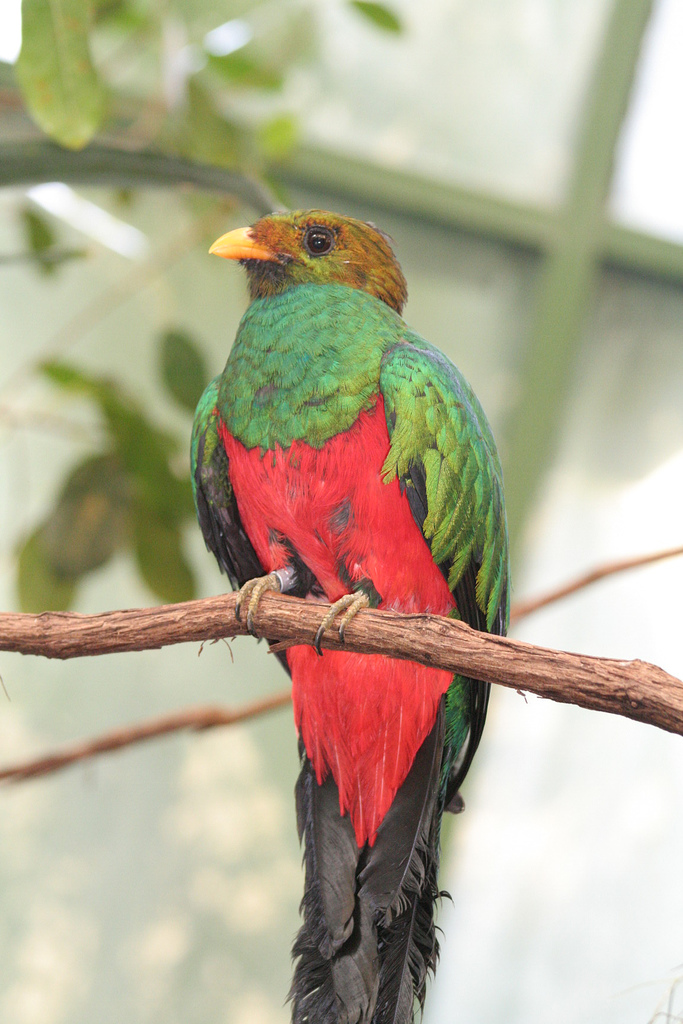
\includegraphics[width=3cm]{figures/quetzal.jpg}
\caption{This is a \textit{quetzal}, which is not a hummingbird.  Compare to the case of the andean ``condor:'' \textit{vultur gryphus.}}
\end{figure}
\end{frame}

\begin{frame}{Vocabulary}
\small
\begin{enumerate}
\item \textbf{Xilo, xiloxochitl}: balsam, balsam tree.  A general term for residue extracted from tree matter that has medicinal properties.  The word balsam comes from The Balm of Gilead, in the Hebrew Bible (Genesis) for a region currently in Jordan.  Why did the Spanish colonials refer to \textit{xilo} as balsam?
\item \textbf{tzipipatli}: an herb native to Nueva Espa\~{n}a used to treat diarrhea.  Compare to how the Europeans treated diarrhea.  What is to be learned from the different treatments?
\end{enumerate}
\end{frame}

\begin{frame}{Vocabulary}
\small
Spanish vocabulary:
\begin{enumerate}
\item \textbf{Sacerdote}: Catholic priest, often used as translators, transcribers, naturalists, and explorers in addition to evangelizing and building churches
\end{enumerate}
\end{frame}

\end{document}